\chapter{Introduction}

Word Sense Disambiguation(WSD) is a notoriously difficult problem in understanding text. Ambiguity is very common in text but humans are so competent at figuring out the word sense from context that most of the time they don't notice the ambiguity in the meaning of the word. Accurate semantic disambiguation would benefit a number of NLP applications; however it is generally acknowledged by WSD researchers that current levels of accuracy need to be improved before WSD technology can be usefully integrated into applications \citep{ide2006making}.

There are two major problems faced by the researchers in this area. One major problem is the dearth of sufficient training data for supervised systems. With a handful of sense-tagged texts currently available, existing WSD systems do not have examples for all the senses of a word most of the times. The other major problem that automatic disambiguation systems face is the fine-grainedness of the sense-distinctions in the sense inventory, WordNet in particular. 

WordNet \citep{miller1995wordnet} \citep{fellbaum1998wordnet} is well known to the Natural Language Processing community as a valuable resource and is one of the most widely used lexical resources. WordNet being a fine grained sense inventory makes it hard even for humans to reliably and consistently distinguish among word senses. In this thesis we would be addressing the latter problem and produce graded word sense relationships which can be used to derive coarse sense clusters with required granularity.

\section{Motivation}

Lets observe the inter-annotator agreement estimates of the data preparation for the Senseval/SemEval tasks on WSD(All Words or Lexical Sample) in table \ref{tab:itaWSD}.

\begin{center}
\begin{longtable}{| c | c | c | c | c | c |}      
    \hline
Workshop and Task & WordNet Version & Verb & Noun & Adjectives & Overall \\\hline 
Senseval-2 AW\footnote{Only approximate information on ITA is available} & \multirow{2}{*}{1.7} & \multirow{2}{*}{70-80} & \multirow{2}{*}{NA} & \multirow{2}{*}{NA} & \multirow{2}{*}{NA} \\ 
\citep{Senseval2AllWordsTask} & & & & & \\ \hline

Senseval-2 LS & \multirow{2}{*}{1.7} & \multirow{2}{*}{NA} & \multirow{2}{*}{86.3} & \multirow{2}{*}{83.4} & \multirow{2}{*}{NA} \\ 
\citep{Senseval2LexicalSampleTask} & & & & & \\ \hline

Senseval-3 AW  & \multirow{2}{*}{1.7.1} & \multirow{2}{*}{67.8} & \multirow{2}{*}{74.9} & \multirow{2}{*}{78.5} & \multirow{2}{*}{72.5}\\ 
\citep{Senseval3AllWordsTask} & & & & & \\ \hline

Senseval-3 LS & \multirow{2}{*}{1.7.1} & \multirow{2}{*}{NA} & \multirow{2}{*}{NA} & \multirow{2}{*}{NA} & \multirow{2}{*}{67.3}\\ 
\citep{Senseval3LexicalSample} & & & & & \\ \hline

Semeval 2007 AW & \multirow{2}{*}{2.1} & \multirow{2}{*}{72} & \multirow{2}{*}{86} & \multirow{2}{*}{NA} & \multirow{2}{*}{NA} \\ 
\citep{Semeval2007WSD} & & & & & \\ \hline
\caption{Inter-annotator agreement for Various Data Preparations} 
\label{tab:itaWSD}
\end{longtable}
\end{center}

As inter-annotator agreement is often considered an upper bound for WSD systems, it is desirable to have a high ITA. \citep{Navigli06meaningfulclustering} believes that a credible upper bound for unrestricted fine-grained WSD is around 70\%, a figure that state-of-the-art automatic systems find difficult to outperform. Therefore it seems that the major bottleneck in effective WSD is the fine grained nature of the WordNet sense inventory, rather than the performance of the best disambiguation systems.

The above points are substantiated by the ITA achieved in preparation of gold standard datasets and performance of the systems in SemEval-2007 Task on Coarse grained WSD \citep{navigli-litkowski:SemEval-2007}. The ITA values on train and test datasets were 86.44\% and 93.80\%. These figures, compared to those in the table \ref{tab:itaWSD}, show that the performance of the WSD systems can be improved by changing the granularity of the adopted sense inventory.

Some of the best systems of SemEval-2007 Coarse Grained WSD task achieved performances in early 80s in the all words task and in the high 80s for the lexical sample task as compared to previous Senseval evaluation exercises, where state-of-the-art systems achieved performance far below 70\%. This encourages us to study in depth the ideas for good sense clustering algorithms and use them to improve the WSD systems so that they can be used in practical scenarios.

\begin{comment}
To understand the granularity of WordNet, lets take an example.
\begin{example}
Consider the senses of the word \textit{evidence} as a \textit{noun} from WordNet version 3.1\footnote{Online WordNet Search: \url{http://wordnetweb.princeton.edu/perl/webwn}} in the table \ref{tab:evidenceExample}.
For most of the applications the sense distinctions are too-fine and are not required. 
One might say that they are all clearly related. \cite{mccarthy2006relating}
\begin{table}[h]
\centering
\begin{tabular}{ | l | p{12cm} |} 
\hline
WordNet Sense & Gloss \\ \hline
evidence\#n\#1 & evidence, grounds (your basis for belief or disbelief; knowledge on which to base belief)  ``the evidence that smoking causes lung cancer is very compelling`` \\ \hline
evidence\#n\#2 & evidence (an indication that makes something evident) ''his trembling was evidence of his fear'' \\ \hline
evidence\#n\#3 & evidence ((law) all the means by which any alleged matter of fact whose truth is investigated at judicial trial is established or disproved) \\ \hline    
\end{tabular}
\caption{Senses of the word \textit{evidence}} 
\label{tab:evidenceExample}
\end{table}
\end{example}
\end{comment}

\section{WordNet}
WordNet \citep{miller1995wordnet} \citep{fellbaum1998wordnet} is a computational lexicon of English based on psycholinguistic principles, created and maintained at Princeton University\footnote{\url{http://wordnet.princeton.edu}}. Nouns, verbs, adjectives and adverbs are grouped into sets of cognitive synonyms (\textit{synsets}), each expressing a distinct concept. These synsets are then interlinked by means of conceptual-semantic and lexical relations. Additionally, a synset contains a brief definition (“gloss”) and, in most cases, one or more short sentences illustrating the use of the synset members. Word forms with several distinct meanings are represented as many distinct synsets. Thus, each form-meaning pair in WordNet is unique. We are using WordNet 3.0, which contains 155,287 words organized in 117,659 synsets. \footnote{\url{http://wordnet.princeton.edu/man/wnstats.7WN.html}} 

\noindent
WordNet relations can be summarised as follows:
\begin{itemize}
\item \textit{Lexical Relations}: Lexical relations connect word senses included in the respective synsets
  \begin{itemize}
  \item \textit{Antonymy}: X is an antonym of Y if it expresses the opposite concept (e.g. \textit{good\#a\#1}\footnote{The format we use to express a word sense is \textit{lemma\#POS\#senseNumber}} is the antonym of \textit{bad\#a\#1})
  \item \textit{Pertainymy}: X is an an adjective which can be defined as ``of or pertaining to'' a noun (e.g. \textit{dental\#a\#1} pertains to \textit{tooth\#n\#1})
  \item \textit{Nominalization}: a noun nominalizes a verb Y (e.g. \textit{service\#n\#2} nominalizes the verb \textit{serve\#v\#4})
  \end{itemize}
\item \textit{Semantic Relations}: Semantic Relations apply to synsets in their entirety
  \begin{itemize}
  \item \textit{Hypernymy-Hyponymy-Troponymy}: The most frequently encoded relation among synsets is the super-subordinate relation (also called IS-A relation).
  Y is a hypernym of X if every X is a (kind of) Y. Hypernymy holds between pairs of nominal and verbal synsets. (for e.g. \textit{motor vehicle\#n\#1} is a hypernym of \textit{car\#n\#1}).
  Hyponymy and Troponymy are the inverse relation of hypernymy for nominal and verbal synsets respectively.
  \item \textit{Meronymy-Holonymy}: Y is a meronym of X if Y is a part of X. (e.g. \textit{flesh\#n\#3} is a meronym of \textit{fruit\#n\#1}.
  Holonymy is the inverse relation of meronymy.
  \item \textit{Entailment}: a verb Y is entailed by a verb X if by doing X you must be doing Y (e.g. \textit{snore\#v\#1 entails sleep\#v\#1})
  \item \textit{Similarity}: an adjective X is similar to an adjective Y (e.g. \textit{beautiful\#a\#1} is similar to \textit{pretty\#a\#1})
  \item \textit{Attribute}: A noun X is an attribute for which an adjective Y expresses a value (e.g. \textit{hot\#a\#1} is a value of \textit{temperature\#n\#1})
  \item \textit{See also}: this is a relation of relatedness between adjectives (e.g \textit{beautiful\#a\#1} is related to \textit{attractive\#a\#1} through the \textit{see also} relation)
  \end{itemize}  
\end{itemize}

Figure \ref{fig:excerptFromWordNet} gives an insight into the relationships contained in WordNet \citep{navigli2009WSDSurvey}.
\begin{figure}[h]
\begin{center}
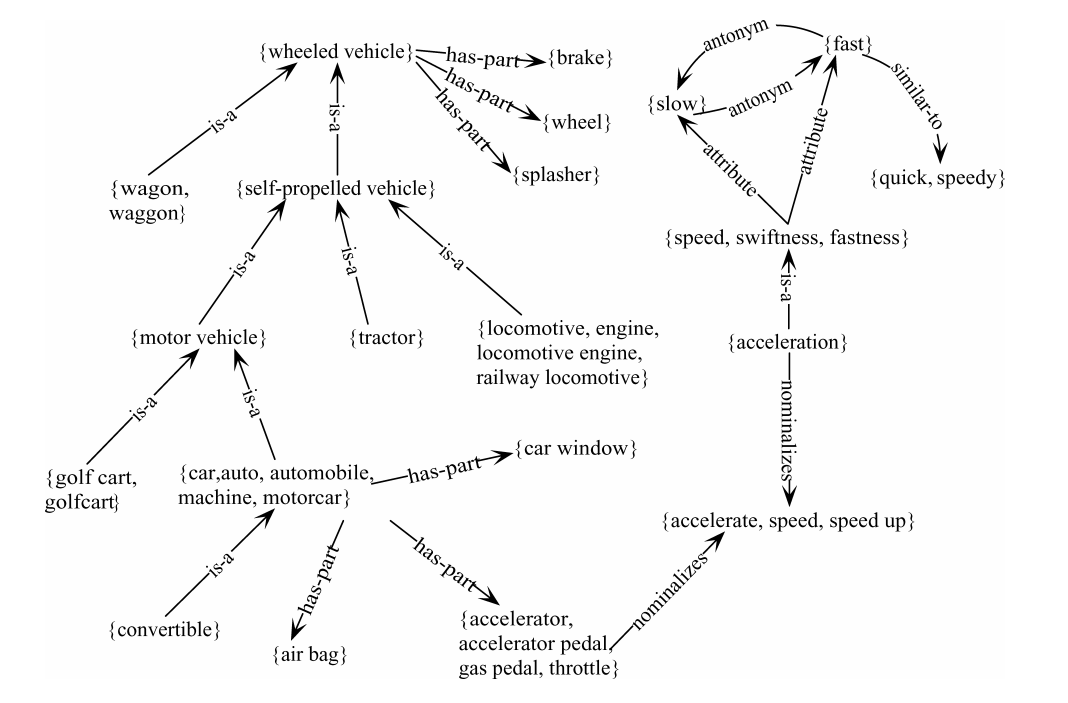
\includegraphics[scale = 0.6]{excerptFromWordNet.png}
\caption{Excerpt From WordNet}
\label{fig:excerptFromWordNet}
\end{center}
\end{figure}

\section{Problem Statement}
%\textit{Can we produce and evaluate coarse-grained sense inventories of arbitrary granularity from lexical resources like WordNet and show ?}

%The problem can be more succinctly defined as follows: Design a system which given a word \textit{w} with its part of speech \textit{p}, lists the senses of the word. The system should be able to control the granularity of sense distinctions.

Formally, the task we are attempting has two objectives: 
\begin{enumerate}
\item Given a fine-grained sense inventory like WordNet, we wish to produce a clustering over WordNet synsets at any arbitrary granularity, which can serve as a coarse sense dictionary. 
\item Given a coarse sense inventory obtained by clustering fine-grained senses, assess its quality and show that it helps boost sense disambiguation on standard test sets.
\end{enumerate}

%\chapter{Background}
\section{Related Work}
\label{chapter:Background}
Systems using WordNet as the underlying ontology often suffer because of the fine-grained nature of the sense inventory. With more and more applications using WordNet, clustering word senses such that the application developer has the control over the granularity becomes very important.

\paragraph{}
One of the earliest attempt at coarsening of Machine Readable dictionaries was made by \citep{Dolan:1994}. 
They attempted to discover sense similarities between senses of Longman's Dictionary of Contemporary English(LDOCE) using multiple heuristics based on a variety of information about a sense's meaning.

\paragraph{}
A wide number of manual and automatic techniques have been proposed since then for clustering sense inventories and creating mappings across sense inventories of different granularities. 
%This chapter talks about the previous attempts to generate coarse senses for words, and the different ideas involved in the same.
%\section{Clustering WordNet Senses}
In this section, we discuss the approaches proposed in literature to coarsen sense inventories. The different ideas to cluster senses can be broadly categorized as follows: 
\begin{itemize}
\item Merging senses based on the sense ontology structure.
\item Clustering based on word sense similarity estimated from external corpora.
\item Exploiting Disagreements: between WSD systems or between human annotators.
\item Translational equivalences of senses in other languages.
\item Manually-annotated or automatically constructed mappings to coarser grained sense inventories.
\item Clustering senses using supervision.
\end{itemize}

\subsection{Merging senses based on ontology structure}
\citep{peters1998automatic} suggest clustering of two word senses based on a wide variety of structural cues from the ontology structure. They cluster senses which are connected by ontology based relations like  \textit{twins}\footnote{Two synsets which share more than one word in their synonym list.}, \textit{autohyponymy}\footnote{If one sense is a direct descendant of the other in the ontology.}, 
\textit{sisters}\footnote{Word senses that share the same hypernym: The sister relation is not limited to two senses, but can also occur between three or more senses of the same word. Sometimes, a particular word exhibits more than one type of sister relation.}, 
\textit{cousins}\footnote{Node pairs whose hyponyms exhibit a specific relation to each other: identified and listed by lexicographers in WordNet 1.5.} etc.
\citep{Mihalcea01ez.wordnet:principles} extended this idea and proposed six semantic principles to merge synsets and probabilistic principles to drop infrequent synsets.
Some interesting principles include merging synsets sharing a \textit{pertainym}, \textit{antonym} or sharing the same \textit{verb group}\footnote{Verb Groups are manually determined by lexicographers.}.
This was the first attempt to group synsets instead of word senses.

\paragraph{}
A number of synset similarity measures based on the WordNet structure have also been proposed in literature like 
Path Based Similarity Measures by \citep{WuPalmer:1994}, \citep{LCH:1998}, Information Content Based Measures by \citep{Resnik:1995}, \citep{JCN:1997}, \citep{Lin:1998} and Gloss Based Heuristics by \citep{Lesk:1986},\citep{Banerjee:2002}. We discuss these similarity measures in detail in Section \ref{section:similarityMeasures}.
Though these measures have not been used directly for WordNet sense clustering, they have motivated researchers in the NLP community to make full use of the WordNet structure to capture similarity between senses.

\subsection{Clustering based on Word Sense similarity estimated from External Corpora}
For estimating similarity between words, many corpus oriented attempts have been made like \citep{Pereira:93a}, \citep{Lin:1998}, \citep{kolb2008disco} and \citep{agirre2009study}. The problem with these approaches is that they are not able to handle the polysemous nature of words. Also, the dearth of sense annotated corpora prevents most of these methods to be used effectively in computing word sense similarities.

\paragraph{}
\citep{agirre2003clustering} associated a topical vector with each word sense, called \textit{Topic Signatures}, whose dimensions are the words in the vocabulary, and the weights try to capture which are the words closer to the target word sense. The cosine similarity between the vectors of two senses is used as the similarity between them. To calculate these vectors, they collect contexts for a polysemous words from manually sense-tagged corpora and by using instances of a polysemous word's monosemous relatives\footnote{Single-sense synsets related by hypernym, hyponym or any other relation of WordNet.} from large untagged corpora and the web. The idea behind the approach is that while related senses may not have a lot of shared contexts directly, because of lack of sense annotated data, they may have semantic associations with the same subset of words that share similar distributional contexts with the target word. By using distributional neighbours from raw text, the method avoids the data sparsity problem.

\paragraph{}
On similar lines is the approach by \citep{mccarthy2006relating}. They use a combination of word-to-word distributional similarity combined with the JCN WordNet based similarity measure \citep{JCN:1997}. They introduce a more relaxed notion of sense relatedness which allows the user to control the granularity for the application in hand.

\subsection{Exploiting Disagreements: between WSD Systems or between Human Annotators}
The central idea involved here is that whenever good WSD systems or human annotators get confused while disambiguating, the senses they mark as answers are semantically related to the correct answer.
\begin{example}
Consider the following noun senses of the word \textit{bass}:
\begin{itemize}
\item bass (the lowest part of the musical range)
\item bass, bass part (the lowest part in polyphonic music)
\item bass, basso (an adult male singer with the lowest voice)
\item sea bass, bass (the lean flesh of a saltwater fish of the family Serranidae)
\item freshwater bass, bass (any of various North American freshwater fish with lean flesh (especially of the genus Micropterus))
\item bass, bass voice, basso (the lowest adult male singing voice)
\item bass (the member with the lowest range of a family of musical instruments)
\item bass (nontechnical name for any of numerous edible marine and freshwater spiny-finned fishes)
\end{itemize}
\end{example}

It is unlikely that a human annotator mistags the musical sense of \textit{bass} with its fish sense. Similar results are expected from a good WSD system as well.

\paragraph{}
\citep{chklovski2003exploiting} derives confusion matrices exploiting the disagreements between human annotators and uses the same to generate coarse sense clusters. On the other hand, \citep{agirre2003clustering} uses the freely available outputs of the WSD systems that participated in Senseval-2 \citep{Edmonds:2001} to construct the confusion matrices between word senses and then cluster them using hierarchial agglomerative clustering. Though promising, these techniques are severely limited by the amount of available manually sense-tagged data and the performance of the WSD systems.

\subsection{Translational Equivalences of Senses in other languages}
\citep{chugur2002polysemy} constructed similarity matrices for Senseval-2 \citep{Edmonds:2001} words using \textbf{translation equivalences} in 4 languages, a method proposed by \citep{resnik1999distinguishing}.
The principle involved can be summed as: \textit{two word senses are deemed similar if they are often translated with the same word in a given context}. Using more than one languages allows the systems to cover as many word sense distinctions as possible. \citep{agirre2003clustering} uses the similarity matrices provided by \citep{chugur2002polysemy} and report resulting hierarchial clusters.

With the advent of WordNets being developed in multiple languages\footnote{GlobalWordNet lists the WordNets available in the public domains: \url{http://www.globalwordnet.org/gwa/wordnet_table.html.}} as well as multilingual ontologies like BabelNet \citep{NavigliPonzetto:12aij}, this seems a promising area which can help in coarsening of senses.


\subsection{Manually-annotated or automatically constructed mappings to coarser grained sense inventories}
Mapping WordNet to other inventories either manually or automatically to generate coarse senses has also been  tried by many researchers in the NLP community. When the different WordNet senses map to the same sense in the other ontology via manual mapping or automatic mapping, it is expected that the senses must have been semanticallyunder the lime light of close. The underlying assumption being that the automatic mapping is able to capture the semantic similarity between the concepts in both the ontologies with high efficacy.

The attempts made in this vein include mapping between WordNet and Hector Lexicon \citep{palmer2007making}, mapping between WordNet and PropBank \citep{palmer2004different} and mapping WordNet to Levin Classes \citep{levin1993english} \citep{palmer2007making}. Most of these mappings are not complete in both directions, which hampers their utility.

The automatic approach presented by \citep{Navigli06meaningfulclustering} for mapping between sense inventories, WordNet to Oxford English Dictionary to be precise, is an elegant approach exploiting similarities in gloss definition and structured relationships in the two sense inventories. The approach can be extended to discover more semantic relationships in WordNet by using the ontology structure of the ontology mapped to WordNet.

\subsection{Clustering senses using supervision}
One of the earliest attempt to cluster senses using supervision was proposed by \citep{snow07mergesense}. They train a Support Vector Machine \citep{vapnikSVM:95} over a wide variety of features derived from WordNet and other lexical resources, whose predictions serve as a distance measure between synsets. Further, for the purpose of sense clustering they assume a zero sense similarity score between synsets with no intersecting words. They cluster synsets using average link agglomerative clustering and the synset similarity model learnt. While merging synsets to construct a coarse taxonomy, they retain only the hypernym ancestry of the sense with the highest frequency in SemCor \citep{SemCor}. They add every other relationship to the new merged sense as long as the acyclic nature of the relations is conserved.

\section{Discussion}
In this section, we discuss some ideas which shaped the direction of our approach to the problem of WordNet sense clustering.

\subsection{Dropping Infrequent WordNet Synsets}
To reduce polysemy in WordNet, \citep{Mihalcea01ez.wordnet:principles} proposed to drop infrequent synsets, along with merging similar senses. They scored the synsets using frequency information of senses in SemCor \citep{SemCor} and dropped the low scoring synsets. 

We study the usefulness of this idea on the SemEval 2007 WSD test datasets \citep{navigli-litkowski:SemEval-2007}, in which we have three generic Wall Street Journal texts and two domain-specific documents (relating to computer programming and Italian painting respectively). Our scoring function is similar to the one proposed by \citep{Mihalcea01ez.wordnet:principles} and is given by:

\begin{equation}
Score(Synset) = \sum_{i \in Synset} Score(WordSense_i) 
\end{equation}

\begin{equation}
Score(WordSense_i) = \frac{Frequency(WordSense_i)+\alpha}{Frequency(LemmaWord_i) + \alpha*NumberOfSenses(LemmaWord_i)} 
\end{equation}

Here $\alpha$ is the Laplacian correction parameter(for our study we take $\alpha=1$).
The scoring function does not make reference to the component word senses directly and thus we do not have to deal with the problem of data sparseness that would result from the limited size of the corpus.

We drop the synsets whose score is less than a threshold and study the number of instances for which the correct answer was removed, thus accounting for error. Since the task was on coarse grained WSD evaluation, we have multiple senses as the correct answer. In this case, we measure the fraction of senses removed from the set of correct senses for each of the instances. We report the error score calculated, weighted by the number of instances in the documents.

\begin{center}
\begin{longtable}{| c | c | c |}  
\hline
\textbf{Corpora Type} & \textbf{Threshold} & \textbf{Weighted Error Score} \\ \hline
WSJ & 0.03 & 7.72 \\ \hline
Domain & 0.03 & 10.48 \\ \hline
WSJ & 0.06 & 13.91 \\ \hline
Domain & 0.06 & 14.19 \\ \hline
WSJ & 0.1 & 18.77 \\ \hline
Domain & 0.1 & 19.13 \\ \hline
\caption{Synsets Dropping Study}
\label{tab:synsetsDroppingStudy}
\end{longtable}
\end{center}

We observe that for lower thresholds, the error rate is higher for domain specific datasets whereas as we increase the threshold, thus removing more and more synsets, the error rates of both the datasets become comparable. The results match our expectation as we expect that some of the words in domain specific datasets would have low frequencies and thus low scores. To summarise, while working with text from the general domain, removing some infrequent synsets might improve the disambiguation but in case of domain specific datasets, it should not be done.

\subsection{Clustering Synsets Vs Clustering Senses}
For generating a coarse sense inventory, many researchers have focused on clustering WordNet senses into groups i.e. generate coarse senses for each word by merging its senses \citep{agirre2003clustering} \citep{chklovski2003exploiting} \citep{Navigli06meaningfulclustering}. In this approach, we would like to highlight two problems. One problem is that to do this a stopping criterion is required such as the number of clusters required for each word. This has been done with the numbers determined by the gold standard for the purposes of evaluation \citep{agirre2003clustering} but ultimately the right number of classes for each word cannot usually be predetermined even if one knows the application, unless only a sample of words are being handled. Therefore such coarsening systems cannot be used to derive coarse senses for all the words and thus are unable to produce coarse sense inventories. The other problem is the inconsistent sense clusters obtained because of independent generation of coarse senses for each word. Even manually done sense clusterings can have this error: consider the sense clusters of the verbs \textit{require} and \textit{need} from Senseval-2 judgements in figure \ref{fig:transitiveError} \citep{snow07mergesense}.

\begin{figure}[h]
\begin{center}
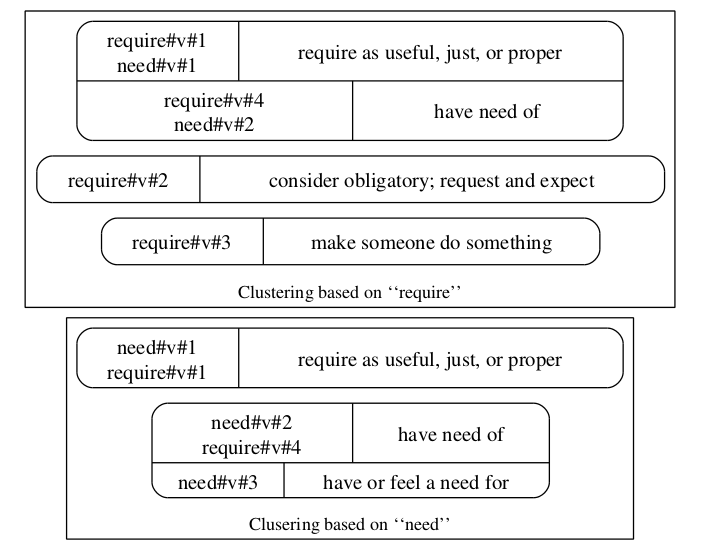
\includegraphics[scale = 0.6]{transitiveError.png}
\caption{Inconsistent sense clusters for the verbs \textit{require} and \textit{need} from Senseval-2 judgements}
\label{fig:transitiveError}
\end{center}
\end{figure}

The two WordNet 2.1 senses \textit{need\#v\#1} and \textit{need\#v\#2} clustered in word specific labelling for \textit{require}, are not clustered according to word-specific labeling for \textit{need}. These transitive closure errors suggest that for deriving consistent coarse senses, we should cluster synsets and not senses.

\section{Evolution of Evaluation Frameworks}
We would like to highlight here the different frameworks used in literature for evaluating the sense clustering problem. Early systems studied the quality of clusters of word senses by studying polysemy degree of the text \citep{Mihalcea01ez.wordnet:principles} or by measuring the entropy and purity of the clusters obtained \citep{agirre2003clustering}.

Another idea is to compare the clustering obtained against a manually sense clustered dataset as done by \citep{chklovski2003exploiting}. This can be done by treating clustering as a pairwise classification task and reporting the F-Score for the classification task. The problem with this approach of evaluation is that in clustering applications often the number of pairs in a cluster is relatively small. This imbalance could lead to understating pairwise similarity and can be avoided by using FScore for both the classes as performance evaluators.

The recent line of thought in evaluation is to go for a task based evaluation. \citep{mccarthy2006relating} studied the performance of first sense heuristics in the Senseval-2 English Lexical Sample Task \citep{Senseval2LexicalSampleTask}. \citep{Navigli06meaningfulclustering} and \citep{snow07mergesense} assess the effect of automatic sense clustering on the three best-ranking WSD systems of the English all-words task at Senseval-3 \citep{Senseval3AllWordsTask}. Since the main reason for building a clustering of WordNet senses is to make WSD a feasible task, studying the performance of WSD systems on coarse sense inventories seems a well founded approach.

\section{Broad Overview of our Approach}
Our approach closely resembles \citep{snow07mergesense} as far as supervised learning of the synset similarity is concerned. But to learn synset similarity of synset pairs which don't share a word, instead of giving them zero similarity, we learn it using a variant of the SimRank framework \citep{Jeh02simrank}. 

Also, \citep{snow07mergesense} proposes to modify the WordNet ontology structure to produce a coarse version of WordNet; however we argue on the lines of \citep{mccarthy2006relating} that we should relate senses as a matter of degree to permit a softer notion of relationships between senses compared to fixed groupings so that the granularity can be varied according to the needs of the application.

\begin{comment}
\subsection{Understanding sense clustering}
When we merge two synsets, should we modify the underlying structure of taxonomy as well?
What should be the repercussion of the mergings on the taxonomy?

An important point to note here is that if we merge two synsets and introduce the merged synsets instead of the original synsets in the WordNet taxonomy, either we'll be adding some spurious relations and/or we'll be losing some relationship information.

\end{comment}

\section{Organization of Thesis}
The rest of this thesis is organized as follows. 
%Chapter \ref{chapter:Background}, reviews the algorithms proposed for the task of sense clustering and the evaluation frameworks for the same. 
Chapter \ref{chapter:SupervisedSynsetSimilarity} discusses a supervised attempt to capture WordNet synset similarity using various features derived from WordNet and external corpora. 
Chapter \ref{chapter:Semi-SupervisedSynsetSimilarity}, presents a semi-supervised approach to estimate WordNet synset similarity using a variant of SimRank \citep{Jeh02simrank} and describes our approach to produce a coarse sense inventory. 
The conclusion and future work are part of chapter \ref{chapter:conclusion}.

